%%%%%%%%%%%%%%%%%%%%%%%%%%%%%%%%%%%%%%%%%%%%%%%%%%%%%%%%%%%%%%%%%%%%%%%%%%%%%%%%%%
\begin{frame}[fragile]\frametitle{}
\begin{center}
{\Large Conclusion}
\end{center}
\end{frame}


%%%%%%%%%%%%%%%%%%%%%%%%%%%%%%%%%%%%%%%%%%%%%%%%%%%%%%%%%%%
\begin{frame}[fragile]\frametitle{Future Techniques}
\begin{center}
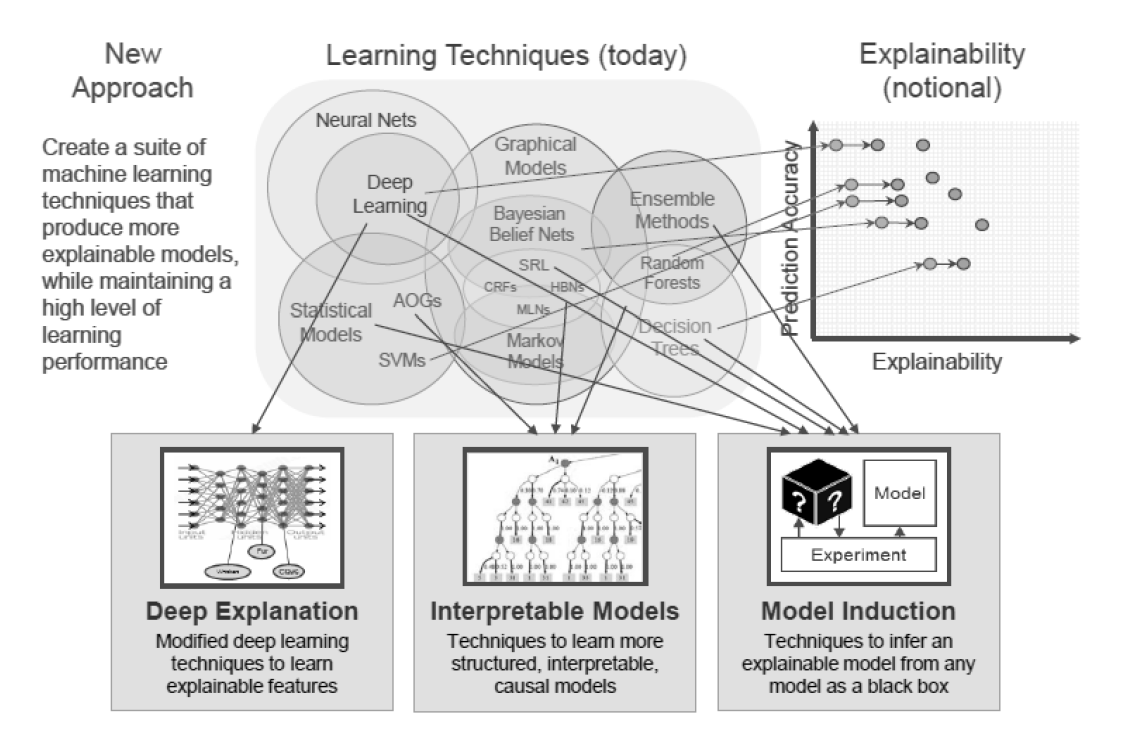
\includegraphics[width=0.8\linewidth,keepaspectratio]{xai22}
\end{center}

\tiny{(Ref:Explainable AI (XAI) – A Perspective, Saurabh Kaushik  )}
\end{frame}

%%%%%%%%%%%%%%%%%%%%%%%%%%%%%%%%%%%%%%%%%%%%%%%%%%%%%%%%%%%
\begin{frame}[fragile]\frametitle{So, Finally \ldots}

\begin{center}
AI is just a set of algorithms, 
which (predominantly ) finds patterns from given Inputs as well as Outputs
\end{center}
\end{frame}

%%%%%%%%%%%%%%%%%%%%%%%%%%%%%%%%%%%%%%%%%%%%%%%%%%%%%%%%%%%
\begin{frame}[fragile]\frametitle{For example: to find out clause ``Term'' \ldots}
\begin{itemize}
\item Need to supply AI algorithm with 100s/1000s of ``Term'' clause samples
\item Gets trained on patterns, word frequencies, context words
\item Stores this information as ``model''
\item Can be used to classify unseen clause, whether ``Term'' or not.
\end{itemize}
\end{frame}

%%%%%%%%%%%%%%%%%%%%%%%%%%%%%%%%%%%%%%%%%%%%%%%%%%%%%%%%%%%
\begin{frame}[fragile]\frametitle{Quiz}
If you want to find something ``new'', what would be needed?
\end{frame}

%%%%%%%%%%%%%%%%%%%%%%%%%%%%%%%%%%%%%%%%%%%%%%%%%%%%%%%%%%%
\begin{frame}[fragile]\frametitle{Summary}
\begin{itemize}
\item AI-ML-DL approaches are non-deterministic (but (\ldots)?)
\item For good results, need good annotated data and lots of it
\item Annotations need to be perfect (``Gold''), else Garbage-In-(\ldots)
\item Data should cover all possible variations
\item AI-ML-DL just fits the data, but just that, it does it automatically!!
\item ML has better explain-ability than DL (why?)
\end{itemize}
\end{frame}

%%%%%%%%%%%%%%%%%%%%%%%%%%%%%%%%%%%%%%%%%%%%%%%%%%%%%%%%%%%
\begin{frame}[fragile]\frametitle{Btw, thoughts to ponder on \ldots}
\begin{itemize}
\item ‘AI is biased'
\item ‘Explainable AI' is to understand how/why it is biased
\item But then \ldots
\item Human are biased too \ldots
\item ‘Explainable Humans'\ldots the next topic?
\end{itemize}
\end{frame}
